\documentclass[a4paper, 11pt]{article}
\usepackage[utf8]{inputenc}
\usepackage[left=18mm, right=18mm, top=22mm, bottom=22mm]{geometry}

\usepackage{amsmath,amsfonts,amssymb,bm}
\usepackage[english]{babel}
\usepackage[hyphens]{url}
\usepackage{hyperref}
\usepackage{xcolor}
\usepackage{fancyhdr}
\usepackage{graphicx}
\usepackage{booktabs}
\usepackage{float}
\usepackage{multirow}
\usepackage{tikz}
\usetikzlibrary{matrix}

% Preferred style, matching docs/pipeline_modules.tex ------------------------
\definecolor{harvardcrimson}{HTML}{8C1D40}
\definecolor{softgrey}{HTML}{F3F3F3}
\definecolor{kwcol}{HTML}{1F4E79}
\definecolor{datablockcol}{HTML}{4B644A}

\hypersetup{
  colorlinks=true,
  linkcolor=harvardcrimson,
  citecolor=harvardcrimson,
  urlcolor=harvardcrimson,
  hypertexnames=false,
}

\pagestyle{fancy}
\fancyhf{}
\rhead{\textcolor{harvardcrimson}{\textbf{GPU cluster pipeline modules}}}
\lhead{\textcolor{harvardcrimson}{\textbf{Arwa}}}
\cfoot{\thepage}
\renewcommand{\headrulewidth}{0.4pt}
\renewcommand{\footrulewidth}{0.4pt}
\setlength{\headheight}{14pt}
\renewcommand{\baselinestretch}{1.12}

% algorithm2e ----------------------------------------------------------------
\usepackage[ruled,vlined,linesnumbered]{algorithm2e}
\SetKwInput{KwData}{Datablock in}
\SetKwInput{KwResult}{Datablock out}
\SetKwInput{KwConfig}{Ini knobs}
\SetKwFor{PerZ}{for each}{do}{end}
\SetKwProg{Fn}{Function}{:}{}
\DontPrintSemicolon

% Custom commands, matching docs/pipeline_modules.tex -------------------------
\newcommand{\lob}{\lambda^{\rm ob}}
\newcommand{\ltr}{\lambda^{\rm tr}}
\newcommand{\zob}{z^{\rm ob}}
\newcommand{\dprj}{\Delta^{\rm prj}}
\newcommand{\xinl}{\xi_{\rm NL}}
\newcommand{\hMpc}{h^{-1}\,\mathrm{Mpc}}
\newcommand{\hMsun}{h^{-1}\,M_{\odot}}
\newcommand{\Sprj}{\Sigma^{\rm prj}}
\newcommand{\DSprj}{\Delta\Sigma^{\rm prj}}
\newcommand{\Bsmall}{B_{\rm small}}
\newcommand{\Blarge}{B_{\rm large}}
\newcommand{\modname}[1]{\textcolor{kwcol}{\texttt{#1}}}
\newcommand{\blk}[1]{\textcolor{datablockcol}{\texttt{#1}}}
\newcommand{\pyfile}[1]{{\small\path{#1}}}

\title{\vspace{-4ex}\huge \textbf{GPU cluster-cosmology pipeline:}\\[0.5ex]
       \Large \textbf{module reference for \texttt{shearTot\_pipeline.ini}}}
\author{Arwa Abdulghafour}
\date{\today}

\begin{document}
\maketitle

\begin{abstract}
This document is the module-by-module reference for the GPU/CUDA test
pipeline \pyfile{cosmosis_tests/gpu_prj_costanzi2026/shearTot_pipeline.ini}:
the eleven modules that take cosmology and mass--observable-relation
parameters and produce cluster number counts and the two-piece
tangential-shear prediction (one-halo + Costanzi-2026 projection term).
It is a companion to \pyfile{docs/pipeline_modules.tex} (the CPU/production
reference by J.\,H.\,Esteves) -- same notation, same style -- but documents
the GPU-specific module set actually exercised by this test pipeline,
including the bugs found and fixed while getting it to run end-to-end (see
\S\ref{sec:gpu_caveats}) and the current, correct build. All GPU modules
live under \pyfile{src/modules/gpu_prj_costanzi2026/} and
\pyfile{src/modules/gpu_modules/}; validation scripts and notebooks live
under \pyfile{cosmosis_tests/gpu_prj_costanzi2026/py_validation/}.
\end{abstract}

\tableofcontents
\vspace{1em}

% ============================================================================
\section{Pipeline topology}
\label{sec:topology}

The module sequence in \pyfile{shearTot_pipeline.ini} is:

\begin{center}
\fbox{\parbox{0.95\linewidth}{\centering
\modname{consistency} $\to$ \modname{camb} $\to$ \modname{mstar} $\to$
\modname{mf\_tinker} $\to$ \modname{prj\_params} $\to$ \modname{halo\_model}
$\to$ \modname{sigmaCritInv} $\to$ \modname{numberCountsFull\_t} $\to$
\modname{shear1hmissel} $\to$ \modname{bselmarggpu} $\to$
\modname{shear\_prj}}}
\end{center}

The \modname{sampler = test} setting runs exactly one sample through this
chain (a ``smoke run''), writing every datablock section to disk under the directory named by
the ini's \texttt{save\_dir} key (\pyfile{outputs/}). There is no \modname{likelihoods} module at
the end of this pipeline (unlike \pyfile{docs/pipeline_modules.tex}'s
production chain) -- this is a wiring/physics test, not an MCMC driver.

\begin{table}[H]
\centering
\small
\begin{tabular}{@{}l l r p{0.37\linewidth}@{}}
\toprule
Module & Type & Timing & Role \\
\midrule
\modname{consistency}       & CSL (Py)      & 3\,ms    & normalise cosmological parameters \\
\modname{camb}               & CSL (Py)      & 1259\,ms & Boltzmann code: linear+nonlinear $P(k,z)$, distances \\
\modname{mstar}              & CSL (Py)      & 78\,ms   & $\sigma(R,z)$ from $P(k,z)$ (feeds the HMF) \\
\modname{mf\_tinker}         & CSL (Fortran) & 98\,ms   & Tinker 2008 halo mass function $dn/d\ln M(M,z)$ \\
\modname{prj\_params}        & local (Py)    & 1\,ms    & Costanzi-2026 EMG richness-projection coefficients \\
\modname{halo\_model}        & local (Py)    & 150\,ms  & $b(M,z)$, $\xinl(r,z)$, optional NFW lensing tables \\
\modname{sigmaCritInv}       & local (Py)    & 2\,ms    & $\langle\Sigma_{\rm crit}^{-1}\rangle(z_L, R)$ \\
\modname{numberCountsFull\_t}& local (CUDA)  & 134\,ms  & $N_i$ cluster number counts \\
\modname{shear1hmissel}      & local (CUDA)  & 303\,ms  & $N_i[\gamma_t^{1h,{\rm full}}](R)$, miscentered \\
\modname{bselmarggpu}        & local (CUDA)  & 3286\,ms & $(P_1,I_1,J)$, $b_{\rm eff}$, $\Bsmall,\Blarge$ (selection bias) \\
\modname{shear\_prj}         & local (CUDA)  & 363\,ms  & two-halo projection $\DSprj(R)$ (rnd$+$cl) \\
\midrule
\multicolumn{2}{r}{\textbf{Total pipeline time:}} & \textbf{5680\,ms} & \\
\bottomrule
\end{tabular}
\caption{Module inventory, with per-module wall time from one
\texttt{sampler=test} run (Artemis A40 GPU,
\pyfile{shearTot_pipeline.ini}) -- a single sample, not an
averaged benchmark, so treat these as indicative, not precise.
\textbf{\modname{bselmarggpu} dominates the runtime}: at $3.29\,$s it is
$\sim 58\%$ of the total $5.68\,$s, roughly $10\times$ the next most
expensive module (\modname{shear1hmissel}, $303\,$ms) -- if this pipeline
ever needs to get faster, this is the module to optimise first. ``CSL'' is
a CosmoSIS-standard-library module (not authored in this repo, described
only briefly here); ``local'' is custom code under this repo. Full theory
+ numerical-recipe detail is given for every local module below; CSL
modules get a one-line role only, per \S\ref{sec:csl_modules}.}
\label{tab:gpu-module-roles}
\end{table}

% ============================================================================
\section{Shared conventions}
\label{sec:conventions}

Same conventions as \pyfile{docs/pipeline_modules.tex} \S\,Shared
conventions -- repeated here for a standalone read.

\paragraph{Units.} All lengths are in $\hMpc$ (comoving, per little-$h$).
$\Sigma,\Delta\Sigma$ are in $\hMsun\,\mathrm{pc}^{-2}$. Halo bias is
dimensionless. Cosmology parameters follow CAMB conventions.

\paragraph{Richness bin convention.} DES-Y3-style richness bin edges are
$[20,30,45,60,200]$ with arithmetic centres $\{25,37.5,52.5,130\}$. Photo-$z$
bins are $[0.20,0.35]\cup[0.35,0.50]\cup[0.50,0.65]$ with midpoints
$\{0.275,0.425,0.575\}$. The full test pipeline (\pyfile{shearTot_pipeline.ini})
sweeps all $4\times 3=12$ bins; \pyfile{shearTot_pipeline.ini}
(the one actually run and referenced throughout this document's worked
numbers) restricts \modname{shear\_prj} to a single bin,
$\lob\in[20,30)$, $\zob\in[0.20,0.35]$, on 5 radii.

\paragraph{Wall grid layout.} Evaluators that produce per-bin observables
read flat 1-D axis arrays from the ini (\texttt{zo\_low}, \texttt{zo\_high},
\texttt{lambda\_bin} or \texttt{lob\_bin\_low}/\texttt{lob\_bin\_high}, and
optionally \texttt{radii}) and zip them index-for-index into grid points
(\pyfile{utils/make_grid_points.hh}, either
\texttt{make\_grid\_points\_wall\_of\_numbers} for
\texttt{use\_cartesian\_product=false} or the cartesian-product variant).
\textbf{Only the cartesian-product path publishes a \blk{gridpoints}
output array} (\pyfile{utils/CosmoSISSICUDAModule.hh}); the zipped path
(used by \modname{shear\_prj}) does not -- reconstructing which grid point
a given \blk{vals[i]} belongs to requires re-reading the ini directly (see
\pyfile{py_validation/check_shear_prj.py::read_ini_wall_grid}).

\paragraph{Mass-axis convention (\modname{mf\_tinker} / \texttt{HMF\_t}).}
CosmoSIS \modname{mf\_tinker} stores \blk{mass\_function/m\_h} in units of
$\Omega_m\cdot\hMsun$. The CUDA \texttt{HMF\_t} constructor
(\pyfile{src/models/hmf_t.cuh}) rescales its internal spline axis by
$\ln(\Omega_m-\Omega_\nu)$ at construction time -- so in principle every
downstream evaluator should query with the raw, unshifted $\ln M$.
\textbf{In practice several evaluators (\modname{numberCountsFull\_t},
\modname{shear1hmissel}, and -- as of the fix in
\S\ref{sec:gpu_caveats} -- \modname{shear\_prj}) do exactly that}, matching
the constructor's own internal convention; this was flagged as a possible
bug in earlier project notes but empirically the ``as-coded'' (unshifted)
convention is what the constructor expects. See
\pyfile{py_validation/check_number_counts.py} for the side-by-side
as-coded-vs-shifted comparison that was used to investigate this.

% ============================================================================
\section{How many integrals run, and how}
\label{sec:integral_count}

\subsection{What a ``grid point'' is}

Each of the four CUDA modules (\modname{numberCountsFull\_t},
\modname{shear1hmissel}, \modname{bselmarggpu}, \modname{shear\_prj})
does not evaluate one integral -- it evaluates \emph{one integral per bin}
of a table. Picture the richness/redshift binning of
\S\ref{sec:conventions} as a table: rows are richness bins, columns are
redshift bins. Fig.~\ref{fig:grid12} is exactly that table for
\modname{numberCountsFull\_t}/\modname{bselmarggpu} -- $4$ richness bins
$\times$ $3$ redshift bins $= 12$ cells. \textbf{Every cell is a separate
integral}: the code cannot compute ``the whole table'' in one integral,
because $K_i$ (the richness-selection kernel, Eq.~\eqref{eq:emg_cdf}) and
$K_j$ (the photo-$z$ kernel) both depend on \emph{which} bin edges are
being integrated against, so a different cell means a genuinely different
integrand.

\begin{figure}[H]
\centering
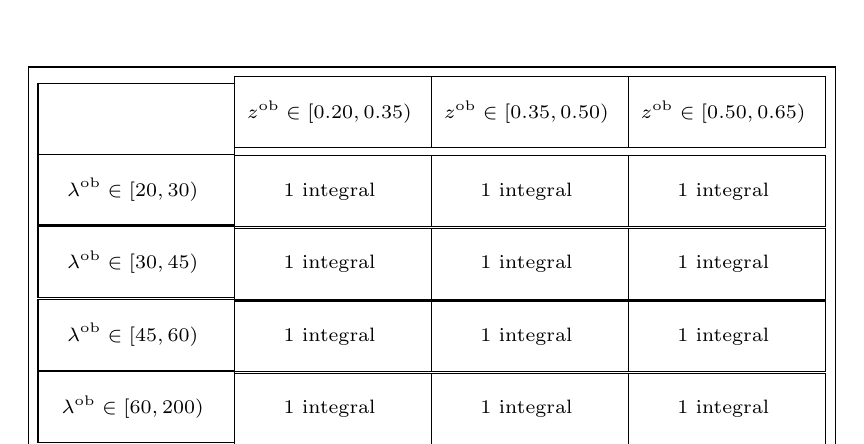
\begin{tikzpicture}[
  every node/.style={draw, minimum width=2.5cm, minimum height=0.9cm,
                      align=center, font=\scriptsize},
]
\matrix (m) [matrix of nodes, nodes in empty cells,
             column sep=-\pgflinewidth, row sep=-\pgflinewidth] {
   & $\zob\in[0.20,0.35)$ & $\zob\in[0.35,0.50)$ & $\zob\in[0.50,0.65)$ \\
  $\lob\in[20,30)$   & 1 integral & 1 integral & 1 integral \\
  $\lob\in[30,45)$   & 1 integral & 1 integral & 1 integral \\
  $\lob\in[45,60)$   & 1 integral & 1 integral & 1 integral \\
  $\lob\in[60,200)$  & 1 integral & 1 integral & 1 integral \\
};
\end{tikzpicture}
\caption{\modname{numberCountsFull\_t} / \modname{bselmarggpu}'s grid: $4$
richness bins $\times$ $3$ redshift bins $= 12$ cells, each cell one
integral (Eq.~\eqref{eq:nc_gpu} / Eq.~\eqref{eq:p1i1j}).}
\label{fig:grid12}
\end{figure}

\modname{shear1hmissel} adds a third axis, radius: the observable is not
``how many clusters'' but ``what is the lensing signal \emph{at radius
$R$}'', so every richness/redshift cell of Fig.~\ref{fig:grid12} is
further split into $5$ radius sub-points ($R\in\{0.5,1,2,5,10\}\,\hMpc$),
giving Fig.~\ref{fig:grid60}: the same $12$ cells, now $5$ integrals each.

\begin{figure}[H]
\centering
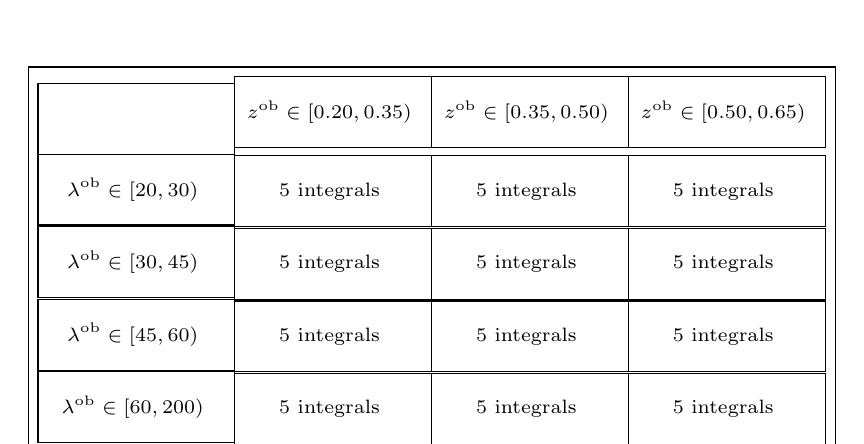
\begin{tikzpicture}[
  every node/.style={draw, minimum width=2.5cm, minimum height=0.9cm,
                      align=center, font=\scriptsize},
]
\matrix (m) [matrix of nodes, nodes in empty cells,
             column sep=-\pgflinewidth, row sep=-\pgflinewidth] {
   & $\zob\in[0.20,0.35)$ & $\zob\in[0.35,0.50)$ & $\zob\in[0.50,0.65)$ \\
  $\lob\in[20,30)$   & 5 integrals & 5 integrals & 5 integrals \\
  $\lob\in[30,45)$   & 5 integrals & 5 integrals & 5 integrals \\
  $\lob\in[45,60)$   & 5 integrals & 5 integrals & 5 integrals \\
  $\lob\in[60,200)$  & 5 integrals & 5 integrals & 5 integrals \\
};
\end{tikzpicture}
\caption{\modname{shear1hmissel}'s grid: same $12$ richness$\times$redshift
cells as Fig.~\ref{fig:grid12}, each now split into $5$ radius sub-points
-- $12\times 5 = 60$ integrals total, one per (richness, redshift, radius)
combination (Eq.~\eqref{eq:shear1h_gpu}).}
\label{fig:grid60}
\end{figure}

\modname{shear\_prj} does \emph{not} follow this clean rectangular-grid
pattern. It runs with \texttt{use\_cartesian\_product=false} (``zipped''
mode, \S\ref{sec:conventions}): rather than covering every combination of
richness $\times$ redshift $\times$ radius, the ini gives a flat, explicit
\emph{list} of $(\lob_{\rm bin}, \zob, R)$ triples to evaluate, and the
code zips them one-for-one. On \pyfile{shearTot_pipeline.ini} that
list has only $5$ entries (one richness/redshift cell, $5$ radii); on the
full \pyfile{shearTot_pipeline.ini} it has $20$ (not the full
$4\times3\times5=60$ a cartesian product would give -- only a
hand-picked subset of richness/redshift/radius triples).

\subsection{How each integral actually runs}

For every cell in the relevant figure above, \pyfile{utils/CosmoSISSICUDAModule.hh}
(the shared ``front-desk'' machinery of \S\ref{sec:gpu_caveats}) does the
same three steps -- already spelled out per-module in the
\texttt{algorithm2e} blocks of \S\ref{sec:number_count_gpu},
\S\ref{sec:shear1h_gpu}, \S\ref{sec:shear_prj_gpu}: (i) look up that
cell's bin edges from the ini, (ii) hand the integrand and those edges to
the PAGANI adaptive GPU cubature (\texttt{eps\_rel}/\texttt{eps\_abs}/\texttt{max\_eval}
control when it stops, \S\ref{sec:gpu_caveats}), (iii) write the resulting
scalar into \blk{vals[i]} at that cell's index. The cells are independent
of each other -- nothing about cell $(\lob=[20,30),\zob=[0.20,0.35))$
depends on any other cell's result -- so in principle they could all run
in parallel; in practice \texttt{CosmoSISSICUDAModule} loops over them one
at a time on a single GPU.

\subsection{Grand total, this pipeline}

\begin{center}
\small
\begin{tabular}{@{}l p{0.24\linewidth} p{0.32\linewidth} r@{}}
\toprule
Module & Grid & Integrals/cell & Total \\
\midrule
\modname{numberCountsFull\_t} & $4\lob\times 3\zob$ & 1 (3-D, Eq.~\eqref{eq:nc_gpu}) & 12 \\
\modname{shear1hmissel}       & $4\lob\times 3\zob\times 5R$ & 1 (3-D, Eq.~\eqref{eq:shear1h_gpu}) & 60 \\
\modname{bselmarggpu}         & $3\zob\times 4\lob$ & 1 shared 4-D pass $\to P_1,I_1,J$ (Eq.~\eqref{eq:p1i1j}) & 12 \\
\modname{shear\_prj}          & 5 hand-picked triples & 1 (3-D, Eq.~\eqref{eq:sigma_prj_gpu}) & 5 \\
\midrule
\multicolumn{3}{r}{\textbf{Total GPU integration calls, this test pipeline:}} & \textbf{89} \\
\bottomrule
\end{tabular}
\end{center}

On the full \pyfile{shearTot_pipeline.ini} (\modname{shear\_prj} at $20$
triples instead of $5$), the same total is $12+60+12+20=104$.
\modname{bselmarggpu}'s $12$ GPU calls are counted once each even though
every call returns three numbers ($P_1,I_1,J$) -- they share a single
integrand evaluation loop (\S\ref{sec:bselmarggpu_gpu}), not three
separate cubature passes.

% ============================================================================
\section{Cosmology background (CSL modules)}
\label{sec:csl_modules}

\modname{consistency}, \modname{camb}, \modname{mstar}, and
\modname{mf\_tinker} are all CosmoSIS-standard-library modules, not authored
in this repo -- they build the ``physical backdrop'' every other module
reads from:

\begin{itemize}
  \setlength\itemsep{2pt}
  \item \modname{consistency} derives a self-consistent cosmological
    parameter set (e.g.\ $\Omega_\Lambda = 1-\Omega_m-\Omega_k$) from
    whatever subset \blk{values\_simple\_gpu.ini} specifies.
  \item \modname{camb} runs the CAMB Boltzmann code (\texttt{mode=all}),
    publishing \blk{matter\_power\_lin}, \blk{matter\_power\_nl}
    (Takahashi halofit), and \blk{distances} ($\chi(z)$, $D_A(z)$).
  \item \modname{mstar} computes $\sigma(R,z)$ (density-field variance
    smoothed on scale $R$) from \blk{matter\_power\_nl}, the input the
    halo mass function needs.
  \item \modname{mf\_tinker} computes $dn/d\ln M(M,z)$ (Tinker et al.\ 2008
    calibration) from $\sigma(R,z)$, publishing \blk{mass\_function/\{m\_h,
    z, dndlnmh\}} -- read directly by \texttt{HMF\_t} (\S\ref{sec:conventions}).
\end{itemize}

None of these four publish anything Costanzi-2026-specific; they are
identical in role to their counterparts in
\pyfile{docs/pipeline_modules.tex} (there named \modname{consistency},
\modname{growth}$+$\modname{cp\_camb}, and \modname{mf\_tinker}).

% ============================================================================
\section{\texttt{prj\_params}: EMG richness-projection coefficients}
\label{sec:prj_params}

\modname{Path:} \pyfile{y3_buzzard/prj_params.py}.

Publishes the 8 Exponentially-Modified-Gaussian (EMG) coefficients
$(a_\tau, b_\tau, a_\mu, b_\mu, a_\sigma, b_\sigma, a_{\rm fprj}, b_{\rm
fprj})$ on a fixed 15-node $z$ grid spanning $[0.10, 0.80]$ in steps of
$0.05$, into \blk{plob\_ltr\_params/\{z, a\_tau, b\_tau, \dots\}}. These are
frozen, hardcoded best-fit values (not re-derived per sample) -- the module
does no cosmology-dependent computation, it is a pure lookup-table loader.
They parametrise the richness-projection kernel

\begin{equation}
\label{eq:emg_cdf}
  P(\lob \le x \,|\, \ltr, z)
  = \Phi(z_{\rm std}) - f_{\rm prj}(\ltr,z)\,
    \exp\!\Big[-\tau(x-\mu) + \tfrac12 \tau^2\sigma^2\Big]\,
    \Phi\!\big(z_{\rm std} - \tau\sigma\big),
\end{equation}
with $z_{\rm std} = (x-\mu)/\sigma$, $\Phi$ the standard normal CDF, and
$(\mu,\sigma,\tau,f_{\rm prj})$ each linearly interpolated in $z$ at fixed
$\ltr_{\rm safe}=\max(\ltr, 0.5)$:
\begin{align}
  \mu &= a_\mu + b_\mu\,\ltr_{\rm safe}, &
  \sigma &= b_\sigma\,\ltr_{\rm safe}^{\,a_\sigma}, \\
  \tau &= b_\tau\,\ltr_{\rm safe}^{-a_\tau}, &
  f_{\rm prj} &= \frac{b_{\rm fprj}}{(1+e^{-\ltr_{\rm safe}})^{a_{\rm fprj}}}.
\end{align}
This is the analytic replacement for the numerically-integrated richness
selection kernel of Costanzi et al.\ 2019 (the \texttt{int\_lc\_lt\_des\_t}
family) -- see \pyfile{src/models/emg_des_t.cuh} for the GPU
implementation and \S\ref{sec:number_count_gpu} / \S\ref{sec:bselmarggpu_gpu}
for its consumers ($K_i$ in \modname{numberCountsFull\_t}, and the
$P(\lob|\ltr,z)$ weight in \modname{bselmarggpu}'s marginalisation).

% ============================================================================
\section{\texttt{halo\_model}: bias, \texorpdfstring{$\xinl$}{xi\_NL}, and optional NFW lensing tables}
\label{sec:halo_model}

\modname{Path:} \pyfile{y3_buzzard/halo_model_cosmosis.py}
(\pyfile{haloModel.py} for the underlying \texttt{biasModel}/\texttt{lensingModel}
classes).

\subsection{Always-on outputs}

Two outputs are published unconditionally (every Costanzi-2026 downstream
consumer needs them):
\begin{itemize}
  \setlength\itemsep{2pt}
  \item \textbf{Halo bias} $b(M,z)$, via peak-height formalism: the bias
    model is built once from \blk{matter\_power\_lin} at $z=0$
    (\texttt{cluster\_toolkit.bias\_at\_nu}), then evaluated at each
    redshift by rescaling the peak height $\nu(M) \to \nu(M)/D(z)$, with
    $D(z)$ the growth factor \emph{renormalised} to $D(0)=1$ (CosmoSIS's
    own \blk{growth\_parameters/d\_z} is un-normalised, $D\to a$ at early
    times -- this module explicitly divides by $D(z{=}0)$ before use).
    Published as \blk{haloModel/bias}, shape $(N_z, N_M)$.
  \item \textbf{Nonlinear matter correlation function} $\xinl(r,z)$, from
    \texttt{cluster\_toolkit.xi.xi\_mm\_at\_r} on a fixed log-spaced
    $r\in[10^{-3},10^{3}]\,\hMpc$, 128-point grid, evaluated per redshift
    slice from \blk{matter\_power\_nl}. Published as \blk{xi\_nl/\{r, z,
    xi\_nl\}}. This is the clustering kernel consumed by
    \modname{bselmarggpu}'s $I_1$/$J$ integrals
    (\S\ref{sec:bselmarggpu_gpu}) and \modname{shear\_prj}'s
    clustering term (\S\ref{sec:shear_prj_gpu}).
\end{itemize}

\subsection{Optional lensing tables}

Two independent ini toggles gate the (expensive) lensing branch:
\texttt{compute\_lensing\_1h} publishes the analytic centred-NFW
$\Sigma_{\rm nfw}(R,M)$/$\Delta\Sigma_{\rm nfw}(R,M)$ tables (cheap,
\texttt{cluster\_toolkit} closed form, needed by \modname{shear1hmissel});
\texttt{compute\_lensing\_2h} additionally publishes the 2-halo
$W_p^{hh}$/$\Sigma_{hh}$/$\Delta\Sigma_{hh}$ tables via a Hankel transform
of $\xi_{mm}$ (the dominant cost of this module, $\sim 200$--$300$\,ms,
\emph{not} needed by the Costanzi-2026 \modname{shear\_prj} path, which
gets its two-halo term from the miscentered-NFW $+\xinl$ construction in
\S\ref{sec:shear_prj_gpu} instead). \pyfile{shearTot_pipeline.ini}
sets \texttt{compute\_lensing\_1h=T}, \texttt{compute\_lensing\_2h=F}: the
1-halo table is needed for \modname{shear1hmissel}, the 2-halo table is
dead weight for this pipeline.

% ============================================================================
\section{\texttt{sigmaCritInv}: lensing efficiency \texorpdfstring{$\langle\Sigma_{\rm crit}^{-1}\rangle(z_L,R)$}{<Sigma\_crit\^{}-1>(zL,R)}}
\label{sec:sigmacritinv}

\modname{Path:} \pyfile{y3_buzzard/buildSigmaCritInv.py}.

\subsection{Model equation}

For a lens at redshift $z_L$ observed against a source population with
redshift distribution $p(z_s)$, the inverse critical surface density
averaged over sources is
\begin{align}
\label{eq:sigma_crit_inv}
  \big\langle \Sigma_{\rm crit}^{-1}(z_L) \big\rangle
  &= \frac{4\pi G}{c^2}\, D_A(z_L)\,(1+z_L)\, \langle\beta(z_L)\rangle, \\
  \beta &\equiv \frac{D_{LS}}{D_S},
\end{align}
with $\langle\beta(z_L)\rangle = \int p(z_s)\, \beta(z_L,z_s)\, dz_s$ a
single number per lens redshift (a statistical average over the ensemble
of sources, not a per-source quantity). The module does \emph{not}
recompute $\beta$ from a redshift distribution at runtime -- it reads a
pre-tabulated $\beta$ lookup table
(\pyfile{data/beta_sigCrit_lut_mock_buzzard_zl.npz}, keys
\texttt{zlens}, \texttt{Radii}, \texttt{zEff}, \texttt{betaEff}) built once
from a fiducial cosmology, and applies a cosmological-shift correction
at run time:
\begin{align}
  \beta(z_L) &= 1 - \frac{s(z_S)}{s(z_L)}\big(1-\beta_{\rm fid}(z_L)\big), \\
  s(z) &\equiv \frac{D_A(z)(1+z)/h}{[D_A(z)(1+z)/h]_{\rm fid}}
  \quad (\texttt{scale\_shift}\ \text{from}\ \modname{halo\_model}),
\end{align}
i.e.\ $\beta_{\rm fid}$ is corrected toward the pipeline's current
cosmology by the ratio of comoving-distance-over-$h$ scale factors between
the current and fiducial runs, rather than re-integrating over the source
distribution every sample -- a lookup-table shortcut, not an approximation
of the physics itself.

\subsection{Output and the \texttt{is\_delta\_sigma} switch}

Publishes \blk{sigmaCritInv/\{r\_sigma, z, sigma\_crit\_inv\}}, shape
$(N_{z_L}, N_R)$, interpolated from the $\beta$-table's own $R$ grid onto
\blk{haloModel/r\_sigma}. If the ini sets \texttt{is\_delta\_sigma=T}, the
whole table is forced to $1$ everywhere (\texttt{sigma\_crit\_inv /
sigma\_crit\_inv}) -- a deliberate hack so that any downstream
``$\times\Sigma_{\rm crit}^{-1}$'' multiplication becomes a no-op and the
published ``shear'' is actually $\Delta\Sigma$.
\pyfile{shearTot_pipeline.ini} sets \texttt{is\_delta\_sigma=F}
(the table is the real lensing-efficiency factor) -- this matters directly
for \S\ref{sec:combination}'s unit bookkeeping.

% ============================================================================
\section{\texttt{numberCountsFull\_t}: cluster number counts \texorpdfstring{$N_i$}{Ni}}
\label{sec:number_count_gpu}

\modname{Path:} \pyfile{src/modules/gpu_prj_costanzi2026/numberCountsFull_t.cu}.
Independent Python cross-check: \pyfile{py_validation/check_number_counts.py}.

\subsection{Model equation}

\begin{multline}
\label{eq:nc_gpu}
  N_i = \int_{\ltr_{\rm lo}}^{\ltr_{\rm hi}} d\ltr
        \int_{z_{\rm lo}}^{z_{\rm hi}} dz
        \int_{\ln M_{\rm lo}}^{\ln M_{\rm hi}} d\ln M\;
        \Omega(z)\,\frac{dV}{d\Omega\,dz}\,n(M,z) \\
        \times\, p_{\rm HOD}(\ltr\,|\,M,z)\, K_i(\ltr,z)\, K_j(z),
\end{multline}
where $\Omega(z)$ is the DES-Y3-fit effective survey solid angle
(\pyfile{src/models/omega_z_des.hh}), $n(M,z)=dn/d\ln M$ is the Tinker
HMF (queried with the raw, unshifted $\ln M$ -- \S\ref{sec:conventions}),
$p_{\rm HOD}(\ltr|M,z)$ is the skew-normal mass--observable relation
(Costanzi et al.\ 2019, Eq.\,B1: a Gaussian in $\ltr$ around a power-law
mean $\ltr_m(M,z)$, with an \texttt{erfc} skew correction), $K_i =
P(\lob_{\rm hi}|\ltr,z)-P(\lob_{\rm lo}|\ltr,z)$ is the EMG richness
kernel of Eq.\,\eqref{eq:emg_cdf}, and $K_j$ is an analytic Gaussian-CDF
difference photo-$z$ kernel (\pyfile{src/models/int_zo_zt_des_t.hh}).

\subsection{Algorithm}

\begin{algorithm}[H]
\caption{\texttt{numberCountsFull\_t} (per grid point $i$)}
\KwConfig{\texttt{ltr\_low/high}, \texttt{zt\_low/high}, \texttt{lnm\_low/high},
 \texttt{lob\_bin\_low/high}, \texttt{zo\_low/high}, \texttt{eps\_rel},
 \texttt{eps\_abs}, \texttt{max\_eval}, \texttt{algorithm=pagani}}
\KwData{\blk{mass\_function}, \blk{distances}, \blk{plob\_ltr\_params},
 mass--observable-relation nuisance parameters (\blk{cluster\_abundance})}
\KwResult{\blk{numbercountsfull\_t/\{vals, gridpoints, errors, status,
 nregions\}}}
Build the 4-D wall grid $(\lob_{\rm lo,i}, \lob_{\rm hi,i}, z^{\rm ob}_{\rm
lo,i}, z^{\rm ob}_{\rm hi,i})$ from the ini (cartesian-product mode: 12
points $=4\lambda\times 3z$ on this pipeline)\;
\For{\rm each grid point $i$}{
  Set the integration volume $[\ltr_{\rm lo},\ltr_{\rm hi}]\times
  [z_{\rm lo},z_{\rm hi}]\times[\ln M_{\rm lo},\ln M_{\rm hi}]$ (same
  volume for every $i$ -- only the integrand's $K_i$/$K_j$ bin edges
  change per grid point)\;
  Run the PAGANI adaptive GPU cubature on Eq.~\eqref{eq:nc_gpu} to
  \texttt{eps\_rel}/\texttt{eps\_abs}, capped at \texttt{max\_eval}
  evaluations\;
  Write \blk{vals[i]}, \blk{errors[i]}, \blk{status[i]}\;
}
\end{algorithm}

\subsection{Numerical recipe / validation note}

The independent Python cross-check (\pyfile{check_number_counts.py}) uses
fixed 48-point Gauss-Legendre quadrature per axis (no PAGANI adaptivity)
and reproduces the C++/CUDA output; it was also used to test the
\S\ref{sec:conventions} mass-shift-convention hypothesis empirically by
running the same integral with and without the $\ln(\Omega_m-\Omega_\nu)$
shift on the HMF query -- the shifted version does \emph{not} match the
GPU output, confirming the unshifted convention is the one actually in
effect (both in the C++ and matching what \texttt{HMF\_t}'s own
constructor already baked into its spline axis).

% ============================================================================
\section{\texttt{shear1hmissel}: one-halo shear numerator \texorpdfstring{$N_i[\gamma_t^{1h}]$}{Ni[gt\^{}1h]}}
\label{sec:shear1h_gpu}

\modname{Path:} \pyfile{src/modules/gpu_prj_costanzi2026/Shear1hMisSel.cu}.
Independent Python cross-check: \pyfile{py_validation/check_shear1h.py}.

\subsection{Model equation}

Identical integrand to \modname{numberCountsFull\_t} (Eq.~\eqref{eq:nc_gpu}),
times one extra radial weight -- the miscentered one-halo shear:
\begin{multline}
\label{eq:shear1h_gpu}
  N_i[\gamma_t^{1h}](R) = \int d\ltr\,dz\,d\ln M\;
    \Omega(z)\,\frac{dV}{d\Omega\,dz}\,n(M,z)\,p_{\rm HOD}\,K_i\,K_j \\
    \times\, \gamma_t^{1h,{\rm full}}(R;M,z),
\end{multline}
\begin{multline}
  \gamma_t^{1h,{\rm full}}(R;M,z) =
  \Big[(1-f_{\rm mis})\,\Delta\Sigma_{\rm NFW}(R,M) \\
       + f_{\rm mis}\,\Delta\Sigma_{\rm mis}(R,M)\Big]\,
  \Sigma_{\rm crit}^{-1}(z,R),
\end{multline}
built from \blk{haloModel/dSigma\_nfw} (the centred table,
\S\ref{sec:halo_model}) and \blk{sigmaCritInv/sigma\_crit\_inv}
(\S\ref{sec:sigmacritinv}); $f_{\rm mis}=0.22$ is the default miscentered
fraction (\pyfile{src/models/gamma_1h_nfw.cuh}). \textbf{Note:}
\pyfile{shearTot_pipeline.ini} does not publish a separate
miscentered $\Delta\Sigma$ table (no \blk{haloModel/dSigma\_mis} section),
so $\Delta\Sigma_{\rm mis}\to\Delta\Sigma_{\rm NFW}$ and the mixture
collapses to just the centred term for this run -- confirmed in
\pyfile{check_shear1h.py}'s output.

\textbf{This module's output is already shear} ($\gamma_t$, via the
$\Sigma_{\rm crit}^{-1}$ multiplication above) -- unlike
\modname{shear\_prj} (\S\ref{sec:shear_prj_gpu}), which publishes
$\Delta\Sigma$. This asymmetry is load-bearing for
\S\ref{sec:combination}.

\subsection{Algorithm}

Same structure as \modname{numberCountsFull\_t}'s algorithm above, on a
5-D wall grid $(\lob_{\rm lo}, \lob_{\rm hi}, z^{\rm ob}_{\rm lo}, z^{\rm
ob}_{\rm hi}, R)$ -- 60 points on the full pipeline
($4\lambda\times 3z\times 5R$), with $R\in\{0.5,1,2,5,10\}\,\hMpc$ repeated
identically across every $(\lob,\zob)$ bin. \blk{gridpoints} is published
(cartesian-product mode), so the $(\lob,\zob,R)$ each \blk{vals[i]}
belongs to can be read straight from the output.

% ============================================================================
\section{\texttt{bselmarggpu}: selection-bias marginalisation}
\label{sec:bselmarggpu_gpu}

\modname{Path:} \pyfile{src/modules/gpu_prj_costanzi2026/shear_prj_module/bSelMargGPU.cu}.

This is the Costanzi-2026 $P[X]$ operator module: it quantifies how
optically selecting clusters by \emph{observed} richness $\lob$ (rather
than a fair sample at fixed halo mass) biases the effective large-scale
clustering of the selected sample. Its outputs (\Bsmall, \Blarge) are
consumed directly by \modname{shear\_prj} (\S\ref{sec:shear_prj_gpu}).

\subsection{The \texorpdfstring{$P_1$, $I_1$, $J$}{P1, I1, J} operators}

For each $(\lob, \zob)$ wall point,
\begin{multline}
\label{eq:p1i1j}
  \{P_1, I_1, J\}(\lob,\zob) = \int d\ltr\,dz\,d\ln M\,d\theta\;
    \ltr\, \mathrm{wt}(z,\zob)\,\frac{dV}{d\Omega\,dz}\,n(M,z) \\
    \times\, p_{\rm HOD}(\ltr|M,z)\, b(M,z)^{\{0,1,1\}}\; f_A(\theta)\,\{1,\xinl\sigma,\xinl(1-\sigma)\},
\end{multline}
i.e.\ three weighted variants of the same 4-D integral share one
integrand evaluation (\pyfile{src/models/p_operator_gpu_t.cuh}): $P_1$
carries no bias/clustering factor, $I_1$ and $J$ both carry $b(M,z)\xinl$
but split the angular sigmoid $\sigma(\theta)$ into its complementary
halves. $f_A(\theta)$ is the fractional area overlap between the target's
and the true-richness cluster's projected exclusion disks, and $\mathrm{wt}$
is the shifted-Poisson MOR of \S\ref{sec:mor_shifted}, \emph{not} the
skew-normal MOR of \S\ref{sec:number_count_gpu} -- these are two
independently calibrated mass--observable relations used in different
parts of the pipeline (see \pyfile{check_bsel.py}'s header comment).

\subsection{\texorpdfstring{$b_{\rm eff}$}{b\_eff}: mass-weighted mean bias}
\label{sec:mor_shifted}

\begin{equation}
  b_{\rm eff}(\lob,\zob) =
  \frac{\int d\ln M\; n(M,\zob)\, p_{\rm shifted\text{-}Poisson}(\lob|M,\zob)\, b(M,\zob)}
       {\int d\ln M\; n(M,\zob)\, p_{\rm shifted\text{-}Poisson}(\lob|M,\zob)},
\end{equation}
trapezoidal in $\ln M$, using the same shifted-Poisson MOR as
Eq.~\eqref{eq:p1i1j} (\pyfile{src/models/mor_shifted_poisson_t.cuh}) --
a continuous shifted-Poisson richness--mass relation (Costanzi-2026),
distinct from the skew-normal MOR used by
\modname{numberCountsFull\_t}/\modname{shear1hmissel}.

\subsection{Selection-bias asymptotes and their marginalisation}

The per-$\ltr$ asymptotes follow the Costanzi-2026 closed form
(\pyfile{src/models/b_sel.cuh}):
\begin{equation}
  I_2 = I_1+J, \qquad
  \Delta^{\rm RND} = P_1 + b_{\rm eff}\, I_2, \qquad
  \delta_{\rm prj} = \frac{\lob-\ltr}{\Delta^{\rm RND}} - 1,
\end{equation}
\begin{equation}
  b_\infty(\lob,\ltr) = b_{\rm eff}\,(1+0.13\,\delta_{\rm prj}), \qquad
  b_0(\lob,\ltr) = \frac{(\lob-\ltr) - P_1 - b_\infty I_1}{J}.
\end{equation}
$\Bsmall,\Blarge$ are then the $\ltr$-marginalised averages of $b_0$,
$b_\infty$ over the true posterior $P(\ltr|\lob,\zob)$:
\begin{equation}
\label{eq:B_marg}
  \{\Bsmall,\Blarge\}(\lob,\zob) =
  \frac{\int_0^{\lob} d\ltr\; P(\ltr|z)\, P(\lob_{\rm bin}|\ltr,z)\; \{b_0,b_\infty\}(\lob,\ltr)}
       {\int_0^{\lob} d\ltr\; P(\ltr|z)\, P(\lob_{\rm bin}|\ltr,z)},
\end{equation}
with $P(\ltr|z) = \int d\ln M\, n(M,z)\, p_{\rm shifted\text{-}Poisson}(\ltr|M,z)$
(mass-marginalised prior, trapezoidal in $\ln M$) and $P(\lob_{\rm
bin}|\ltr,z) = P(\lob\le\lob_{\rm hi}|\ltr,z) - P(\lob\le\lob_{\rm
lo}|\ltr,z)$ the EMG kernel of Eq.~\eqref{eq:emg_cdf} evaluated at the
\emph{bin edges} (not just the centre).

\paragraph{Fix applied 2026-07-07 (documented in-code).} An earlier
version of Eq.~\eqref{eq:B_marg} weighted each $\ltr$ sample by
$p_{\rm HOD}(\ltr\,|\,M{=}10^{14}, z)$ -- a single hardcoded representative
mass, independent of $\lob$ and not actually conditioned on $\lob$ beyond
capping $\ltr\le\lob$. Because that fixed-mass profile peaks near
$\ltr\sim 14$ regardless of richness bin, higher-$\lob$ bins ended up
averaging almost entirely over $\delta_{\rm prj}\gtrsim 5$ -- well outside
the range the linear $b_\infty(\delta_{\rm prj})$ relation was calibrated
against (arXiv:2604.05833 Figs.\,6--7 only extend to $\delta_{\rm prj}\sim
5$), producing $\Blarge/b_{\rm eff}$ ratios of $1.7$--$3.2$ instead of the
paper's $\sim 0.8$--$2.0$. Replacing the weight with the proper
$P(\ltr|z)\,P(\lob_{\rm bin}|\ltr,z)$ posterior of Eq.~\eqref{eq:B_marg}
fixed this (\pyfile{bSelMargGPU.cu}, \texttt{compute\_B\_marginalised}).
This EMG evaluation runs on the \emph{host} (not the GPU integrand), via a
plain-host reimplementation of \pyfile{src/models/emg_des_t.cuh}'s
\texttt{cdf()} -- the original class stores \texttt{quad::Interp1D}
members that hold device pointers and segfault if constructed/evaluated
from host code.

% ============================================================================
\section{\texttt{shear\_prj}: two-halo projection term}
\label{sec:shear_prj_gpu}

\modname{Path:} \pyfile{src/modules/gpu_prj_costanzi2026/shear_prj_module/ShearPrjEvaluator_t.cu}
+ \pyfile{sigma_prj_gpu_t.cuh}. Independent Python cross-check:
\pyfile{py_validation/check_shear_prj.py} (plots:
\pyfile{check_shear_prj_plots.ipynb}).

\subsection{Model equation}

\begin{multline}
\label{eq:sigma_prj_gpu}
  \Sprj(R \,|\, \lob, \zob)
  = \int d\theta\,\sin\theta \int dz\, \frac{dV}{d\Omega\,dz}\, w_z(z,\zob)
    \int d\ln M\, n(M,z) \\
    \times\, \Big[\,1 + b(M,z)\, b_{\rm sel}(\theta)\, \xinl(z,\zob,\theta)\,\Big]\,
    \Sigma_{\rm mis}(R \,|\, M, z, \theta),
\end{multline}
same structure and same caveats as documented in
\pyfile{validation_report.tex} \S\,Shear Projection Module -- repeated
here for completeness. $w_z(z,\zob)=\max(0,1-u^2)$, $u=(z-\zob)/\sigma_{\rm
photoz}(z)$, is the photo-$z$ window (\pyfile{src/models/sigma_photoz_table_t.cuh}).
$b_{\rm sel}(\theta) = \Bsmall + (\Blarge-\Bsmall)\,\sigma_{\rm sig}(\theta)$
is the analytic sigmoid closure with $\Bsmall,\Blarge$ read from
\modname{bselmarggpu}'s output (\S\ref{sec:bselmarggpu_gpu}), nearest-neighbour
matched in $(\lob,\zob)$. $\Sigma_{\rm mis}$ is the single-kernel
(\S\ref{sec:shear_prj_gpu}, ``off-centred NFW'' below) miscentered NFW
surface density with the line-of-sight angle $\theta$ itself as the
miscentering offset $R_{\rm mis}=\theta D_A(\zob)$ -- a $\delta$-function
kernel, deliberately \emph{not} the Rayleigh offset
\modname{shear1hmissel} uses for its centred-cluster $f_{\rm mis}$
mixture, because here $\theta$ is already an explicit integration
variable (a convolved offset on top would double-count it). The exclusion
angle gating the $[b\,b_{\rm sel}\,\xinl]$ bracket is $\theta_{\rm
excl}(z)$, $\cos\theta_{\rm excl}(z) = (\chi_z^2+\chi_o^2-R_{\rm
excl}^2)/(2\chi_z\chi_o)$, $R_{\rm excl}=R_\lambda(\lob)(1+\zob)$.

\subsection{Off-centred NFW normalisation}

\begin{align}
  \Sigma_{\rm mis}(r,r_{\rm mis}|M,z) &=
    2\,r_s\,\delta_c\,\rho_{\rm crit}\,\rho_{\rm mult}\,
    u_{\rm NFW}(\log(r/r_s),\log(r_{\rm mis}/r_s)), \\
  \delta_c &= \frac{200}{3}\frac{c^3}{\ln(1+c)-c/(1+c)},
\end{align}
$c=4$ fixed, $u_{\rm NFW}$ a pre-tabulated 2-D lookup
(\pyfile{data/nfw_off_center/table_*_single_*}, Wright \& Brainerd
2000 normalisation). $\rho_{\rm mult}=\Omega_m$ (rho-mean convention,
matching the CPU reference and the Python NFW model) -- \textbf{as of the
fix in \S\ref{sec:gpu_caveats}}; the GPU CUDA classes
(\pyfile{src/models/nfw_sigma_mis.cuh}/\pyfile{nfw_dsigma_mis.cuh})
did not carry this multiplier at all until this pipeline was debugged.

\subsection{Algorithm}

\begin{algorithm}[H]
\caption{\texttt{shear\_prj} (per grid point)}
\KwConfig{\texttt{theta\_low/high}, \texttt{zt\_low/high}, \texttt{lnm\_low/high},
 \texttt{lambda\_bin}, \texttt{zo\_low/high}, \texttt{radii},
 \texttt{use\_cartesian\_product=false}, \texttt{eps\_rel}, \texttt{eps\_abs},
 \texttt{max\_eval}, \texttt{algorithm=pagani}}
\KwData{\blk{haloModel/bias}, \blk{xi\_nl}, \blk{distances/d\_c},
 \blk{b\_sel\_marginalised/\{lob,zob,b\_small,b\_large\}}, NFW off-centred
 tables (on disk)}
\KwResult{\blk{shear\_prj/\{vals, errors, probs, status, nregions\}}
 \emph{only} -- see caveats below}
Zip \texttt{lambda\_bin}/\texttt{zo\_low}/\texttt{zo\_high}/\texttt{radii}
index-for-index into the wall grid (zipped mode -- \emph{no}
\blk{gridpoints} output, \S\ref{sec:conventions})\;
\For{\rm each grid point $(\lob_{\rm bin}, \zob, R)$}{
  Look up nearest-$(\lob,\zob)$ $\Bsmall,\Blarge$ from
  \blk{b\_sel\_marginalised}\;
  Run PAGANI over $(\theta, z, \ln M)$ evaluating
  Eq.~\eqref{eq:sigma_prj_gpu}'s full bracketed integrand in one pass
  (\texttt{DSigmaTotalWeight}, \S\ref{sec:gpu_caveats})\;
  Write \blk{vals[i]}\;
}
\end{algorithm}

\subsection{Caveats specific to this module}
\label{sec:shear_prj_caveats}

\begin{itemize}
  \setlength\itemsep{2pt}
  \item \textbf{Output is $\Delta\Sigma$, not shear.} There is no
    $\Sigma_{\rm crit}^{-1}$ multiplication anywhere in this module
    (unlike \modname{shear1hmissel}, \S\ref{sec:shear1h_gpu}) -- despite
    the name, \blk{shear\_prj/vals} must be multiplied by
    \blk{sigmaCritInv/sigma\_crit\_inv} before it can be added to a shear
    quantity. See \S\ref{sec:combination}.
  \item \textbf{Only one combined output, not the CPU's 9-way split.} The
    CPU reference (\pyfile{src/models/sigma_prj_t.hh::ShearPrjEvaluator})
    publishes $\{\Sprj,\DSprj,\gamma_t^{\rm prj}\}\times\{{\rm vals, rnd,
    cl}\}$ (9 outputs). This GPU module publishes a single
    \blk{shear\_prj/vals} = the full bracketed integral of
    Eq.~\eqref{eq:sigma_prj_gpu} (rnd$+$cl combined, since the
    \texttt{DSigmaTotalWeight} fix -- \S\ref{sec:gpu_caveats}); the
    rnd/cl decomposition is only reproducible on the Python side
    (\pyfile{check_shear_prj.py::integrand_dsigma_rnd} vs
    \texttt{integrand\_dsigma\_total}), not as separate C++ outputs.
  \item \textbf{Concentration and mass-shift conventions unverified.} $c=4$
    is hardcoded on both CPU and GPU sides, versus $c=5$ in the Python
    richness-selection reference (per project notes); the HMF
    mass-shift convention (\S\ref{sec:conventions}) has not been
    specifically checked for this module the way it was for
    \modname{numberCountsFull\_t}.
\end{itemize}

% ============================================================================
\section{Observables and the shear composition}
\label{sec:combination}

The theoretical tangential shear prediction is the sum of the two
lensing modules, matching \pyfile{docs/pipeline_modules.tex} Eq.\,(gt\_sum)
and the comment in \pyfile{shearTot_pipeline.ini}:
\begin{align}
\label{eq:gt_sum_gpu}
  \gamma_t^{\rm theory}(R \,|\, i)
  &= \langle\gamma_t^{1h}\rangle_i(R) \;+\; \gamma_t^{\rm prj}(R\,|\,\lob,\zob), \\[4pt]
  \langle\gamma_t^{1h}\rangle_i(R) &= \frac{\blk{shear1hmissel/vals}}{\blk{numbercountsfull\_t/vals}}, \\[4pt]
  \gamma_t^{\rm prj}(R\,|\,\lob,\zob) &= \blk{shear\_prj/vals}(R) \,\times\, \blk{sigmaCritInv/sigma\_crit\_inv}(\zob, R).
\end{align}

\textbf{The $\Sigma_{\rm crit}^{-1}$ factor on the second term is not
optional bookkeeping -- it is required for the sum to be dimensionally
correct.} $\blk{shear1hmissel/vals}/\blk{numbercountsfull\_t/vals}$ is
already shear (the $\Sigma_{\rm crit}^{-1}$ multiplication happens inside
\modname{shear1hmissel}, \S\ref{sec:shear1h_gpu}), but
$\blk{shear\_prj/vals}$ is $\Delta\Sigma$
(\S\ref{sec:shear_prj_caveats}); naively adding the two mixes units. This
was verified numerically (\pyfile{check_shear_prj_plots.ipynb}, ``Plot
-- combined theory shear'' cell): on the single bin this test pipeline
covers ($20\le\lob<30$, $0.20\le\zob<0.35$), $\langle\gamma_t^{1h}\rangle$
dominates and falls steeply at small $R$ (typical NFW cusp behaviour),
while $\gamma_t^{\rm prj}$ is comparatively flat and becomes the
\emph{larger} contributor beyond $R\sim 7$--$8\,\hMpc$ -- exactly the
qualitative picture Costanzi et al.\ 2026 describe for the projection
correction relative to the one-halo term.

% ============================================================================
\section{GPU-specific bugs found and fixed}
\label{sec:gpu_caveats}

Getting this pipeline to run end-to-end (as of the runs referenced
throughout this document) required fixing four issues, none of which
exist in \pyfile{docs/pipeline_modules.tex}'s CPU reference -- they are
specific to the CUDA port:

\begin{enumerate}
  \setlength\itemsep{3pt}
  \item \textbf{Build failure -- wrong include path.}
    \pyfile{ShearPrjEvaluator_t.cu} included
    \pyfile{"models/sigma_prj_gpu_t.cuh"}, a path that does not exist
    (the header lives next to the \texttt{.cu} file). Fixed to a
    same-directory include.
  \item \textbf{Missing $\rho_{\rm mean}$ normalisation.} The CUDA
    \pyfile{NFW_SIGMA_MIS}/\pyfile{NFW_DSIGMA_MIS} classes
    (\pyfile{nfw_sigma_mis.cuh}, \pyfile{nfw_dsigma_mis.cuh}) never had
    the \pyfile{_rho_mult} member their CPU counterparts have, so
    \modname{shear\_prj}'s \texttt{set\_rho\_mult(omega\_m\_)} calls were
    commented out (would not compile) and $\Sigma_{\rm mis}$ was always
    computed at $\rho_{\rm mult}=1$ ($\rho_{\rm crit}$) -- $\Omega_m
    \approx 0.286\times$ too large. Added the member to both CUDA
    classes; re-enabled the calls.
  \item \textbf{Runtime crash at \texttt{setup()}.}
    \pyfile{utils/CosmoSISSICUDAModule.hh} read
    \texttt{max\_eval}/\texttt{eps\_rel}/\texttt{eps\_abs} via a direct
    \texttt{cfg.view\textless{}double\textgreater{}()}, no int/double fallback. Some ini scalars
    (e.g.\ \texttt{max\_eval\,=\,100000}) land in the DataBlock typed as
    \texttt{int}; the direct \texttt{view\textless{}double\textgreater{}()} then threw
    \texttt{cosmosis::Entry::BadEntry}, uncatchable by the constructor's
    function-try-block, aborting the process. Fixed with the same
    int-or-double fallback \pyfile{get_vector_double} already uses for
    array-valued parameters.
  \item \textbf{Selection-bias clustering term computed then discarded.}
    \modname{shear\_prj} was originally built as
    \texttt{SigmaPrjGPU\textless{}DSigmaRndWeight\textgreater{}} -- the ``1$+$'' (uncorrelated)
    term of Eq.~\eqref{eq:sigma_prj_gpu} only. The $b(M,z)\,b_{\rm
    sel}(\theta)\,\xinl$ clustering term \emph{was} computed inside
    \texttt{SigmaPrjGPU::operator()} (guarded by $\theta_{\rm excl}(z)$)
    but discarded by \texttt{DSigmaRndWeight::apply()} -- meaning the
    module's published output carried none of the Costanzi-2026
    selection-bias correction, the paper's central contribution, despite
    computing all the pieces needed for it. Added a
    \texttt{DSigmaTotalWeight} functor that applies the full
    $[1+b\,b_{\rm sel}\,\xinl]$ bracket in one pass, and switched
    \pyfile{ShearPrjEvaluator_t.cu} to use it.
\end{enumerate}

Items 1--3 are infrastructure/robustness fixes -- they change whether the
pipeline runs at all, not the physics. Items 2 and 4 are the physically
significant fixes: item 2 changes the overall normalisation by a factor
of $\Omega_m$; item 4 changes which physics is actually being computed
(background-only vs.\ the full selection-bias-corrected projection term).

% ============================================================================
\section{Summary}

\begin{center}
\small
\begin{tabular}{@{}l p{0.62\linewidth}@{}}
\toprule
Module & Status (this pipeline) \\
\midrule
\modname{consistency}/\modname{camb}/\modname{mstar}/\modname{mf\_tinker} & CSL, unmodified, working \\
\modname{prj\_params}      & working, static lookup table \\
\modname{halo\_model}      & working (1h lensing on, 2h off for this pipeline) \\
\modname{sigmaCritInv}     & working, \texttt{is\_delta\_sigma=F} (real shear conversion) \\
\modname{numberCountsFull\_t} & working, validated to $<1\%$ against independent Python \\
\modname{shear1hmissel}    & working, validated to $<1\%$ against independent Python \\
\modname{bselmarggpu}      & working, marginalisation bug fixed 2026-07-07 \\
\modname{shear\_prj}       & working after 4 fixes (\S\ref{sec:gpu_caveats}); combined-shear
  behaviour matches the paper's qualitative picture; absolute-value
  cross-check against the paper still open \\
\bottomrule
\end{tabular}
\end{center}

% ============================================================================
\begin{thebibliography}{9}
\bibitem{costanzi26} Costanzi, M., Wu, H.-Y., Esteves, J.~H., Grandis, S., To, C., Aguena, M., et al.\ 2026, ``A forward analytical model for the optical selection bias on galaxy cluster lensing profiles,'' arXiv:2604.05833.
\bibitem{costanzi19} Costanzi, M. et al.\ 2019, MNRAS, 482, 490.
\bibitem{wright_brainerd2000} Wright, C.~O.\ \& Brainerd, T.~G.\ 2000, ApJ, 534, 34.
\bibitem{tinker08} Tinker, J. et al.\ 2008, ApJ, 688, 709 -- halo mass function calibration used by \modname{mf\_tinker}.
\end{thebibliography}

\end{document}
